\subsection{Logarithmusfunktion}

\parbox[t]{0.4\textwidth}{
    \underline{Logarithmusfunktion}: 

    \scalebox{0.8}{
        \begin{tikzpicture}
            \begin{axis}[
                axis lines=middle,
                xlabel={$x$},
                ylabel={$y$},
                title={Funktion: $f(x) = ln(x)$},
                %grid=major,
                domain=-2:2, % Range for x
                samples=100, % Number of samples for smoothness
                ]
                \addplot[blue, thick] {ln(x)};
                %\legend{$y = e^x$}
            \end{axis}
        \end{tikzpicture}
    }
}
\hfill
\parbox[t]{0.4\textwidth}{
    \underline{E-Funktionen im vergleich zu Logarithmusfunktion}

    \scalebox{0.8}{
        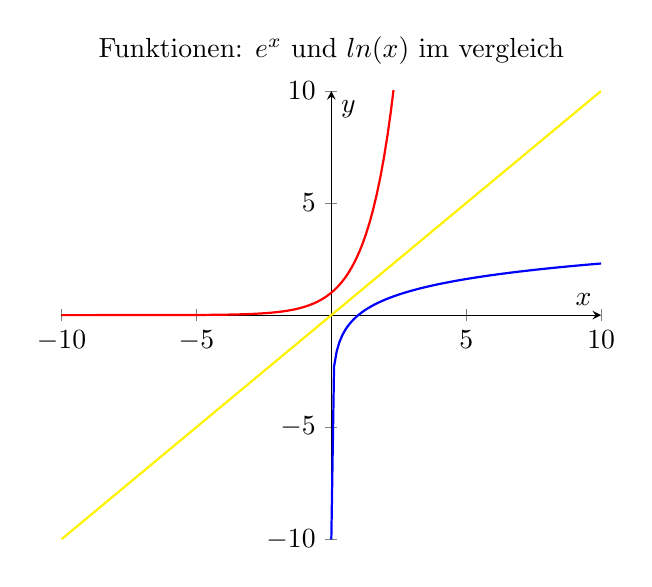
\begin{tikzpicture}
            \begin{axis}[
                axis lines=middle,
                xlabel={$x$},
                ylabel={$y$},
                title={Funktionen: $e^x$ und $ln(x)$ im vergleich},
                %grid=major,
                %domain=-10:10, % Range for x
                xmin=-10,xmax=10,
                ymin=-10,ymax=10,
                samples=100, % Number of samples for smoothness
                ]
                \addplot[blue, thick, domain=exp(-10):10] {ln(x)};
                \addplot[red, thick, domain=-10:3] {exp(x)};
                \addplot[yellow, thick, domain=-10:10] {x};
                %\legend{$y = e^x$}
            \end{axis}
        \end{tikzpicture}
    }
}

